\chapter{Introducción Específica}

\label{Capitulo2}

En este capítulo se desglosan las diferentes herramientas tanto de hardware como software, elegidas para el desarrollo del robot propuesto.

\section{Robot Operating System}

Típicamente denominado ROS, es un framework de robótica de código abierto, el cual fue diseñado originalmente para robots de uso académico. Sin embargo, al día de hoy su uso se ha extendido tanto a la industria como al público aficionado.\newline
ROS ofrece un variado set de herramientas que facilitan las tareas del roboticista en tareas tales como paso de mensajes, computación distribuida e implementación de algoritmos para aplicaciones robóticas.

\subsection{Organización de archivos}

Es adecuado considerar a ROS como algo más que un framework de desarrollo y referirnos a el como un meta-sistema-operativo, ya que ofrece no solo herramientas y librerías sino también funciones similares a las de un sistema operativo. Entre ellas, podemos citar su abstracción del hardware, manejo de paquetes y un completo \textit{toolchain} de compilación. Así también, tal como en un sistema operativo ``real'', los archivos que componen ROS se encuentran organizados en el disco duro de una manera particular, la cual se expresa en la figura \ref{fig:rosSistemaDeArchivos}.

\begin{figure}[ht]
    \centering
    \def\svgwidth{350pt}
    \input{./Figures/estructura_archivos_ros.pdf_tex}
    \caption{Organización de archivos en ROS}
    \label{fig:rosSistemaDeArchivos}
\end{figure}

\newpage
A continuación se detalla en qué consiste cada uno de los bloques que la componen:
\begin{itemize}
    \item \textbf{Paquetes}: Los paquetes de ROS representan la unidad básica de sofware en la plataforma. Estos contienen uno o mas programas de ROS (nodos), librerías, archivos de configuración, etc, los cuales son organizados como una unidad coherente.
    \item \textbf{Manifiesto del paquete}: Esta representado por un archivo único dentro del paquete y el mismo contiene información sobre el mismo tal como el nombre, autor, tipo de licencia, dependencias, banderas de compilación, etc. El archivo \file{package.xml} encontrado en la raíz del paquete es el manifiesto del mismo.
    \item \textbf{Metapaquete}: Es un paquete que hace referencia a uno o mas paquetes usualmente relacionados entre sí, pero sin estar necesariamente acoplados fuertemente unos con otros. El software proveído con este proyecto es un metapaquete.
    \item \textbf{Manifiesto del metapaquete}: Similar al manifiesto del paquete, con la diferencia que el mismo puede incluir dependencias a de tiempo de ejecución hacia otros paquetes.
    \item \textbf{Mensajes}: Representados con la extensión \file{.msg}, son los tipos de datos utilizados por ROS internamente para comunicar los distintos procesos entre sí. El usuario puede definir tipos de mensajes personalizados con campos adaptados a sus necesidades en del directorio \file{msg} dentro del paquete.
    \item  \textbf{Servicios}: Representados con la extensión \file{.srv}, representan interacciones del tipo solicitud/respuesta entre distintos procesos. Los formatos tanto para solicitud como para respuesta pueden definirse en el directorio \file{srv} dentro del paquete.
    \item \textbf{Repositorios}: La gran mayoría de los paquetes de ROS son mantenidos utilizando un sistema de control de versiones (SCV) tales como Git, Mercurial o SVN. Es común encontrar metapaquetes definidos dentro de un mismo único repositorio, el cual es el caso para el repositorio proveído en este trabajo.
\end{itemize}

\subsection{Arquitectura interna}
ROS esta construido sobre una arquitectura basada en grafos, esto significa que las tareas de cómputo son realizadas a través de una red de procesos llamados nodos. Esta red es denominada \textit{Computation Graph} o grafo de cómputo.\newline
Los principales componentes de este grafo son los nodos, el \textit{master} o maestro, el \textit{parameter server} o servidor de parámetros, además de los mensajes, tópicos, servicios y \textit{bags} o bolsas. Cada uno de estos elementos contribuye al funcionamiento del Computation Graph con una funcionalidad específica. Los elementos que lo componen, mostrados en la figura \ref{fig:computationGraph}, se describen a continuación:

\newpage

\begin{figure}[ht]
    \centering
    \def\svgwidth{350pt}
    \input{./Figures/ros_computation_graph.pdf_tex}
    \caption{Estructura del \textit{Computation Graph} de ROS}
    \label{fig:computationGraph}
\end{figure}

\begin{itemize}
    \item \textbf{Nodos}: Son los procesos que realizan las tareas de cómputo dentro del robot, los cuales pueden comunicarse unos con otros a través de la API de ROS. Esto resulta particularmente útil cuando distintos nodos necesitan compartir información entre si. En ROS se fomenta el uso de múltiples nodos que realicen procesos sencillos por sobre procesos grandes y complejos que abarquen toda la funcionalidad.
    \item \textbf{Master}: El ROS Master se encarga de buscar y registrar los diferentes componentes que interactúan en el sisteam. Esto posibilita que diferentes nodos sean capaces de ``encontrarse'' mutuamente, intercambiar mensajes o invocar servicios. En un sistema distribuido, el master debe ejecutarse solamente en una de las computadoras.
    \item \textbf{Servidor de parámetros}: El servidor de parámetros o \textit{parameter server}, permite mantener la información utilizada en configuración de los nodos almacenada en una ubicación central. Esto permite a cada uno de los nodos a acceder y modificar dichos valores.
    \item \textbf{Mensajes}: Los nodos se comunican entre si mediante mensajes, estructuras de datos cuyos campos pueden editarse y permiten ser enviados entre si. Existen tipos de mensajes estandares (enteros, flotantes, booleanos, etc.) así como también es posible definir mensajes propios, adaptados a las necesidades de la aplicación.
    \item \textbf{Tópicos}: Cada mensaje en ROS es transportado utilizando buses llamados tópicos. Cuando un nodo envía un mensaje a través de un tópico, se puede decir que el nodo esta ``publicando un tópico''. Así mismo cuando un nodo recibe un mensaje a través de un tópico, se puede decir que el nodo esta ``subscripto al tópico''. El nodo publicante y el suscriptor no tienen información sobre su mutua existencia, por lo que es posible que existan nodos publicando a tópicos sin suscriptores o viceversa, nodos suscriptos a tópicos sin publicantes.
    \item \textbf{Servicios}: En determinadas aplicaciones, el mecanismo de publicador/suscriptor definido en el ítem anterior podría no ser adecuado. Por ejemplo, en ciertos casos es necesaria una interacción del tipo solicitud/respuesta. En dichas situaciones un nodo podría solicitar la ejecución de un procedimiento rápido por parte de otro nodo y el envío de una respesta con el resultado de dicho cálculo.
    \item \textbf{Logging}: ROS provee un sistema de registro o \textit{logging} denominada Rosbag (bolsa), la cual se utiliza para almacenar información publicada en los tópicos activos, como por ejemplo la proveniente de un sensor que podría ser difícil de generar una y otra vez, pero que a su vez resulta necesaria para depurar determinados algoritmos. Un rosbag permitiría en este caso, generar la información una única vez para luego reproducirla como si fuese una grabación las veces que resulte necesaria.
\end{itemize}

\subsection{Herramienta RViz}

La herramienta RViz (o ROS Visualization tool), es la herramienta oficial de visualización ROS, la cual permite representar de manera gráfica la información transmitida a través de los distintos tópicos. Posee soporte nativo para la mayoría de los mensajes estándar y permite además, expandir su funcionamiento mediante \textit{plugins} los que posiblitan visualizar mensajes personalizados, entre otros.\newline
RViz permite visualizar la representación física del robot, de modo a analizar su configuración de articulaciones (o \textit{joints}) y enlaces (o \textit{links}), como se muestra en la figura \ref{fig:rviz}.

\begin{figure}[ht]
	\centering
	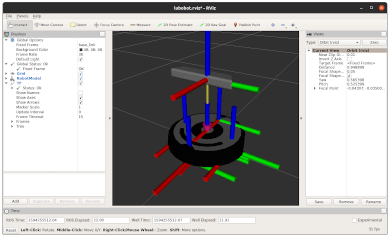
\includegraphics{./Figures/rviz.png}
	\caption{Interfaz gráfica de RViz mostrando los links y joints del robot Lubobot.}
	\label{fig:rviz}
\end{figure}

\subsection{Formato universal de descripción de robots URDF}

El formato universal de descripción de robots o \textit{Universal Robot Description System}, comunmente referido como URDF es un formato estándar para representación de modelos que contengan múltiples piezas conectadas entre sí, como es el caso de los brazos robóticos o líneas de ensamblaje. El mismo es ampliamente utilizado dentro del ecosistema de ROS, plataforma donde vio su origen aunque al día de hoy su uso se ha extendido a otras herramientas fuera del mismo.

\subsection{Librería rosserial}
\subsection{Paquete de navegación ros\_navigation\_stack}
\section{iRobot Roomba 500}
\subsection{Consideraciones}
\section{Placa de desarrollo STM32-NUCLEO}
\subsection{Descripción}
\subsection{Consideraciones}
\section{Sensor Kinect 360}
\subsection{Descripción}
\subsection{Comparación con otras cámaras de profundidad}
\section{Unidad de medición inercial MPU6050}
\subsection{Descripción}
\subsection{Comparación con otras IMU}
